\documentclass[11pt]{article}
\usepackage[margin=0.8in]{geometry}
\usepackage{amsmath,amssymb,booktabs,longtable,graphicx,hyperref}
\hypersetup{colorlinks=true,urlcolor=blue,linkcolor=blue,hypertexnames=false}
\setlength{\emergencystretch}{3em}
\title{Benchmark-Relative Systematic Portfolio Construction:\\An Independent Ten-ETF Historical Study}
\author{Aniket Bhardwaj}
\date{9 October 2026}
\begin{document}
\maketitle
\noindent\textbf{Independent research; not peer reviewed. Retrospective pseudo-out-of-sample evidence.}
\begin{abstract}
This study examines how benchmark-relative tracking-error and turnover limits
compress a fixed composite of momentum, low-volatility and short-term reversal
preferences in a surviving ten-ETF panel. Monthly portfolios are compared with
a monthly 60/40 policy, equal weight and inverse volatility, with a conservative
two-session information lag. Development, validation and final holdout periods
are separated, and the protocol and dataset are frozen before constructed
holdout portfolio performance is examined. Negative outcomes and interrupted
paths remain part of the evidence. After inspecting development/validation
execution failures, formation reserves were introduced and the corrected
specification was frozen before holdout. The 8\% and 12\% TE configurations have
essentially identical performance; turnover was more restrictive under the
tested settings, without establishing a general ranking of portfolio constraints.
Exact-input reproduction requires the original, non-public market-data bundle;
fresh retrieval supports approximate replication on a potentially revised vintage.
Signal capture measures preference expression,
not predictive skill. The results below distinguish arithmetic active returns,
compounded performance and descriptive block-bootstrap uncertainty; they do not
establish persistent alpha or causal effects of volatility regimes.
In the final holdout, the primary model's net CAGR is 13.72\% versus 12.33\% for the frictionless policy. Annualized arithmetic active return is 1.23\% with a descriptive 95\% block interval [-1.55\%, 3.90\%]. Weekly execution failures in development and validation remain part of the robustness evidence.
\end{abstract}
\section{Introduction and research questions}
How do benchmark risk and trading constraints affect signal expression? Does
increased expression improve net historical performance? Can a tighter
tracking-error budget during high policy volatility materially change outcomes?
The policy is a proposed comparison, not a claim of historical optimality.
The original deterministic synthetic study remains unchanged and separate.
\section{Literature review}
Ledoit and Wolf motivate shrinkage risk estimation \cite{lw}; their covariance
result does not establish profitability of this ETF strategy. DeMiguel,
Garlappi and Uppal motivate a transparent equal-weight comparison \cite{dgu}.
Their conclusions concern different universes and estimation problems.
Block resampling recognizes serial dependence rather than treating daily
observations as independent \cite{kunsch}. This study applies those methodological
ideas to portfolio construction without claiming a new asset-pricing discovery.
Momentum research documents winner--loser persistence in individual stocks
\cite{jt}; volatility-return research studies stock-level aggregate and
idiosyncratic risk \cite{ang}; reversal research considers short-horizon
contrarian stock returns \cite{lehmann}. These findings motivate preferences,
not calibrated ETF expected returns. Total ETF volatility is not idiosyncratic
stock volatility, and a 21-session reversal score is not a replication of a
weekly stock-reversal study. Economic portability is an empirical question.
\section{Historical dataset and data quality}
The ordered universe is SPY, IWM, EFA, EEM, IEF, TLT, LQD, HYG, GLD and VNQ.
Equity covers the first four; fixed income covers IEF, TLT, LQD and HYG;
gold and real estate are separate constraint groups. VNQ is treated as a separate
real-estate allocation despite its equity-like risk. Funds were selected
retrospectively and survived to retrieval: this is not an unbiased historical
investable universe. Every fund existed before January 2009; issuer inception
and first-listing sources are recorded in the provenance appendix document.
GLD's November 18, 2004 availability date is its first trading date, distinct
from the trust's November 12 formation date.

The TigZig public API supplies Yahoo Finance data via yfinance. Its documented
auto-adjusted Close incorporates splits and distributions \cite{tigzig}.
The action ledger is preserved without a second adjustment. The operator's
terms describe educational/demonstration use and disclaim accuracy \cite{terms};
an institutional licence and upstream redistribution permission are not claimed.
Raw responses remain outside Git. Adjusted returns approximate total returns
with provider reinvestment conventions; tax and exact distribution reinvestment
execution are not modelled. Latest-vintage revisions can differ from historical
information available at each date.

Validation checks hashes, strict timestamp order, duplicates, positive finite
prices, common NYSE sessions, per-fund availability, distributions/splits,
20\% absolute daily-return review thresholds, original-response Close values,
and actions from a second endpoint of the same provider. The second endpoint
is not an independent market-data validation.

The panel contains 4,463 common sessions from January 2, 2009 to September 30, 2026, with 0 missing sessions and 0 threshold exceedances. The ledger contains 1,133 distributions and no splits in this window; GLD has no cash distributions.


\section{Mathematical model}
With score $s$, benchmark $b$, annual covariance $\Sigma$ and known lagged
holdings $w^{\rm known}$, the existing convex program solves
\[
\max_w\ s^\top w-10(w-b)^\top\Sigma(w-b)
       -0.1\lVert w-w^{\rm known}\rVert_1.
\]
Fully invested long-only portfolios satisfy $\mathbf{1}^\top w=1$ and
$0\leq w_i\leq0.35$. At execution, annual estimated TE is at most 8\%
(5\% in the high-state alternative), absolute active group exposure is at most
10 percentage points, and $T=\tfrac12\lVert w-w^{\rm pretrade}\rVert_1\leq0.30$.
Every accepted solution is independently checked. Infeasible or inaccurate
solver outcomes stop a path rather than silently relaxing constraints.

At return date $t$, signal and decision information end at $t-2$; target weights
are formed then, modelled at close $t-1$, and earn returns after that close.
Execution-close drift changes actual turnover but does not change target
formation. Holdings drift as
\[
w_{i,t}^{\rm end}=\frac{w_{i,t}(1+r_{i,t})}{1+w_t^\top r_t},\qquad
R_t^{\rm net}=w_t^\top r_t-\frac{c}{10000}T_t.
\]
The additive fee convention is a declared NAV approximation; this does not
prove closing prices were executable. Exact share/cash accounting is omitted.
\section{Signals and covariance methodology}
For information date $u$, raw momentum is $P_{u-21}/P_{u-252}-1$;
low volatility is the negative sample standard deviation of the last 63 daily
returns; reversal is $-(P_u/P_{u-21}-1)$. Cross-sectional 5th/95th winsorization
and population-standard-deviation standardization precede the composite
$s=z_{\rm momentum}+z_{\rm lowvol}+0.5z_{\rm reversal}$.
Coefficients are fixed preferences, not calibrated expected returns.
Covariance uses 252 trailing returns, Ledoit--Wolf shrinkage, a $10^{-10}$
daily diagonal ridge and annualization 252. Sample covariance is a declared
robustness alternative. Forward IC is Spearman correlation with subsequent
asset returns through the next rebalance; the terminal period can be partial.

Signal capture is $(w-b)^\top s$ divided by the expression of a same-score,
same-information long-only reference with the 35\% position cap but without
TE, group, turnover constraints or penalties. Exposure is measured against
the realized execution benchmark for both paths. Absolute reference exposure
at most $10^{-10}$ yields an undefined observation. Different ablations have
different reference scores, so their capture ratios are not cardinal skill
comparisons. High capture does not imply superior returns.
\section{Policy benchmark and constraints}
The policy weights, in universe order, are
$(0.30,0.05,0.15,0.10,0.20,0.05,0.15,0,0,0)$.
It resets at the close immediately before the first observed session return
of each month and drifts between resets. The schedule is independently
represented when the active strategy rebalances weekly. Ordinary policy,
equal-weight and inverse-volatility comparisons satisfy their own rules and
portfolio accounting; active-manager TE, sector and turnover mandates are
not imposed on them. Both frictionless and independently cost-adjusted
policy returns are exported. Each independent period starts endowed at
its execution-date policy holdings; the active transition is charged and
the initial policy endowment is not charged.

\subsection{Pre-holdout design revision after execution failures}
Original development/validation active paths without reserves failed execution
checks, predominantly turnover limits following unobserved one-session drift;
those failures remain archived. After inspecting these development/validation
outcomes, Codex introduced identical formation reserves across
active scenarios: 2 percentage points of turnover, 1 percentage point of group
exposure and 0.1 percentage point of annual TE. Thus primary formation caps are
28\%, 9 percentage points and 7.9\%; the high-state formation TE cap is 4.9\%.
Execution mandates remain 30\%, 10 percentage points and 8\%/5\%, respectively.
This is an outcome-informed engineering correction to the initial specification.
The corrected specification was reviewed and frozen before constructed holdout
portfolio performance was examined; published results use that corrected model.
Reserves address engineering feasibility and do not guarantee that execution
constraints remain feasible. Remaining weekly sector failures in development
and validation were retained. A benchmark target
fits the 35\% cap; transition constraints can still be infeasible.
\section{Experiment design and holdout protocol}
Warmup is January 2009--December 2010; development is January 3, 2011--December
29, 2017; validation is January 2, 2018--December 30, 2022; final holdout is
January 3, 2023--September 30, 2026. Models receive physical price slices
ending at each period boundary. Before holdout, data checks, tests,
development/validation review and the configuration were frozen with dataset
hashes and a code commit. An exclusive access ledger was written before
the single final evaluation. No favourable ablation was substituted for
the primary model. Inherited source discovery and issuer verification exposed
incidental holdout-era quotes/performance panels, and full prices were ingested
for quality checks; constructed holdout performance was not used for selection.
The historical split is retrospective, not prospective preregistration.

Experiments A--G cover TE caps 4/8/12\%; turnover caps 10/30/50\%; identical-trade
cost sensitivities 0/10/25/40 bps; fixed 8\% versus normal 8\%/high 5\% TE;
three signal omissions plus regime awareness; the five portfolio strategies;
and sample covariance, three-session information delay and weekly rebalancing.
The full ledgers retain failures. Cost assumptions do not reoptimize holdings.
Metrics use 252 observations/year and sample return standard deviations;
Sharpe/Sortino assume zero risk-free return. Undefined metrics are explicit.

Uncertainty uses circular 21-session blocks, 2,000 resamples, seed 20261008 and
95\% percentile intervals for annualized arithmetic active means. Strategy
differences are paired on the same dates. Approximate within-period stationarity
and dependence within blocks are assumed; structural breaks, longer regime
persistence and multiple comparisons are not resolved. No naive independent-day
significance tests or persistent-alpha conclusions are made.
\section{Empirical performance results}
All returns below are computed from executed paths. CAGR, annualized arithmetic
active return and TE are distinct quantities. Active returns use the frictionless
policy; a cost-adjusted policy comparison is included in the machine-readable
tables. Percent figures are expressed in percentage points.

\subsection{Development}

\begin{center}\small\begin{tabular}{lrrrrr}\toprule Strategy & Gross CAGR & Net CAGR & TE & Active & MDD\\\midrule

Policy (net) & 7.987 & 7.976 & 0.004 & -0.011 & -11.373\\

Equal weight & 6.879 & 6.859 & 2.462 & -1.082 & -11.692\\

Inverse volatility & 6.439 & 6.384 & 4.355 & -1.697 & -9.245\\

Fixed risk & 7.722 & 7.499 & 3.653 & -0.380 & -17.784\\

Regime aware & 7.710 & 7.486 & 3.626 & -0.396 & -17.440\\

\bottomrule\end{tabular}\end{center}

Fixed-risk arithmetic active return is -0.38\% with a 95\% block interval [-3.14\%, 2.08\%]. Mean capture is 0.665, with 84 valid and 0 excluded rebalance observations. Mean forward IC is 0.012. Frictionless policy CAGR is 7.99\%; independently cost-adjusted policy CAGR is 7.98\%.

\subsection{Validation}

\begin{center}\small\begin{tabular}{lrrrrr}\toprule Strategy & Gross CAGR & Net CAGR & TE & Active & MDD\\\midrule

Policy (net) & 3.284 & 3.271 & 0.004 & -0.013 & -24.271\\

Equal weight & 2.766 & 2.743 & 2.752 & -0.618 & -24.064\\

Inverse volatility & 1.461 & 1.400 & 5.436 & -2.228 & -22.547\\

Fixed risk & 2.283 & 2.033 & 3.294 & -1.148 & -25.315\\

Regime aware & 2.330 & 2.086 & 3.250 & -1.093 & -25.315\\

\bottomrule\end{tabular}\end{center}

Fixed-risk arithmetic active return is -1.15\% with a 95\% block interval [-3.67\%, 1.36\%]. Mean capture is 0.548, with 60 valid and 0 excluded rebalance observations. Mean forward IC is -0.060. Frictionless policy CAGR is 3.28\%; independently cost-adjusted policy CAGR is 3.27\%.

\subsection{Holdout}

\begin{center}\small\begin{tabular}{lrrrrr}\toprule Strategy & Gross CAGR & Net CAGR & TE & Active & MDD\\\midrule

Policy (net) & 12.325 & 12.315 & 0.003 & -0.009 & -9.729\\

Equal weight & 11.405 & 11.379 & 2.841 & -0.853 & -9.785\\

Inverse volatility & 9.093 & 9.034 & 3.746 & -3.160 & -8.347\\

Fixed risk & 13.980 & 13.717 & 2.782 & 1.233 & -11.089\\

Regime aware & 13.964 & 13.700 & 2.773 & 1.218 & -11.089\\

\bottomrule\end{tabular}\end{center}

Fixed-risk arithmetic active return is 1.23\% with a 95\% block interval [-1.55\%, 3.90\%]. Mean capture is 0.730, with 45 valid and 0 excluded rebalance observations. Mean forward IC is -0.019. Frictionless policy CAGR is 12.33\%; independently cost-adjusted policy CAGR is 12.32\%.


\section{Constraint sensitivity findings}
Table \ref{allresults} reports every declared scenario. Relaxing a risk cap need
not change an allocation when another constraint or the objective dominates.
The 8\% and 12\% TE configurations have essentially identical performance,
consistent with largely non-binding TE caps at those settings. Turnover restricted
signal expression more than the tested 4\%--12\% TE range under this model,
objective, universe and other constraints. This conditional sensitivity does not
establish that turnover is generally more important than tracking error in
portfolio management. Higher capture does not establish better returns.
Capture and turnover frontiers describe construction mechanics rather than
investment skill. Formation reserves apply identically across frontier scenarios;
10/30/50\% turnover mandates imply 8/28/48\% formation caps.
\section{Volatility-regime comparison}
The classifier uses the monthly-policy return history: trailing 63-session
sample volatility times $\sqrt{252}$, compared with the expanding 75th percentile
of strictly earlier valid rolling observations, requiring 252 earlier values.
Only strict exceedances are high; ties are normal. Labels used in allocation are
dated at the lagged information close and budgets change at rebalances.
The timeline shows observation-date labels, whose availability is after that
close. Conditional results use daily lagged labels and arithmetic summaries;
they do not compound discontinuous subsequences or imply regime causality.

Development: regime-aware minus fixed annualized arithmetic return -0.02\%; paired 95\% block interval [-0.12\%, 0.10\%].


Validation: regime-aware minus fixed annualized arithmetic return 0.05\%; paired 95\% block interval [-0.07\%, 0.18\%].


Holdout: regime-aware minus fixed annualized arithmetic return -0.02\%; paired 95\% block interval [-0.10\%, 0.05\%].


\begin{center}\small\begin{longtable}{lllrrr}\toprule Period & Strategy & State & Days & Active & TE\\\midrule

development & Fixed risk & normal & 1607 & -0.561 & 3.241\\

development & Fixed risk & high & 154 & 1.507 & 6.577\\

development & Regime aware & normal & 1607 & -0.581 & 3.246\\

development & Regime aware & high & 154 & 1.532 & 6.372\\

validation & Fixed risk & normal & 810 & -0.755 & 2.786\\

validation & Fixed risk & high & 449 & -1.855 & 4.056\\

validation & Regime aware & normal & 810 & -0.686 & 2.767\\

validation & Regime aware & high & 449 & -1.827 & 3.979\\

holdout & Fixed risk & normal & 722 & 1.506 & 2.545\\

holdout & Fixed risk & high & 217 & 0.328 & 3.461\\

holdout & Regime aware & normal & 722 & 1.512 & 2.541\\

holdout & Regime aware & high & 217 & 0.241 & 3.439\\

\bottomrule\end{longtable}\end{center}


\section{Robustness and ablation results}
The alternative covariance, delayed-information and signal-omission experiments
remain separately labelled. They are descriptive checks, not an uncontrolled
parameter search. Weekly paths that breach execution constraints receive no
full-period CAGR or fabricated continuation. The omission plots preserve the
full original model rather than selecting the best historical omission.
\section{Economic interpretation}
Costs mechanically reduce net wealth on an unchanged trade path. A stronger
preference alignment can coexist with underperformance, because standardized
signal scores are not expected-return forecasts. Changes in relative performance
across historical periods can reflect asset-class composition, macroeconomic
exposures, estimator error and noise. No regression-based risk-adjusted alpha,
causal regime effect or investable closing-auction advantage is established.
\section{Limitations}
The surviving universe, latest adjustment vintage and Yahoo-derived data are
material selection and measurement limitations. ETF prices embed fund expenses;
taxes, share-lot/cash execution, market impact, liquidity, funding and settlement
are omitted. Turnover is half-L1 and fees are additive fractions of beginning NAV.
Constraints hold at accepted rebalances; drift can violate limits between them,
and realized TE can exceed ex-ante caps. Fixed risk reserves cannot guarantee
future mandate compliance. The modest fixed panel and multiple comparisons limit
generalization; block intervals do not solve structural-break uncertainty.
Zero-rate Sharpe is not a comparison with historical cash yields. The split is
retrospective and independently reproduced source prices can change vintage.
The original market-data bundle is retained locally and is not publicly
available. Fingerprints establish identity but cannot supply those inputs;
exact external reproduction is therefore conditional on original-bundle access.
Fresh downloads can support method replication while changing numerical findings.
\section{Conclusion}
The empirical workflow provides auditable evidence of portfolio-construction
tradeoffs under declared benchmark risk, trading and cost conventions. It also
preserves failed transitions and inconclusive uncertainty. Under the tested model
and parameter range, turnover restricted signal expression more than the TE
range, whose 8\% and 12\% caps were largely non-binding. This is not a general
ranking of portfolio constraints. The reserves were an engineering correction
informed by development/validation failures and frozen before holdout. Signal expression is
a construction diagnostic; these historical results do not establish persistent
alpha. Prospective evaluation and independently licensed institutional data would
strengthen further research.

\clearpage\section*{Research figures}

\begin{figure}[htbp]\centering
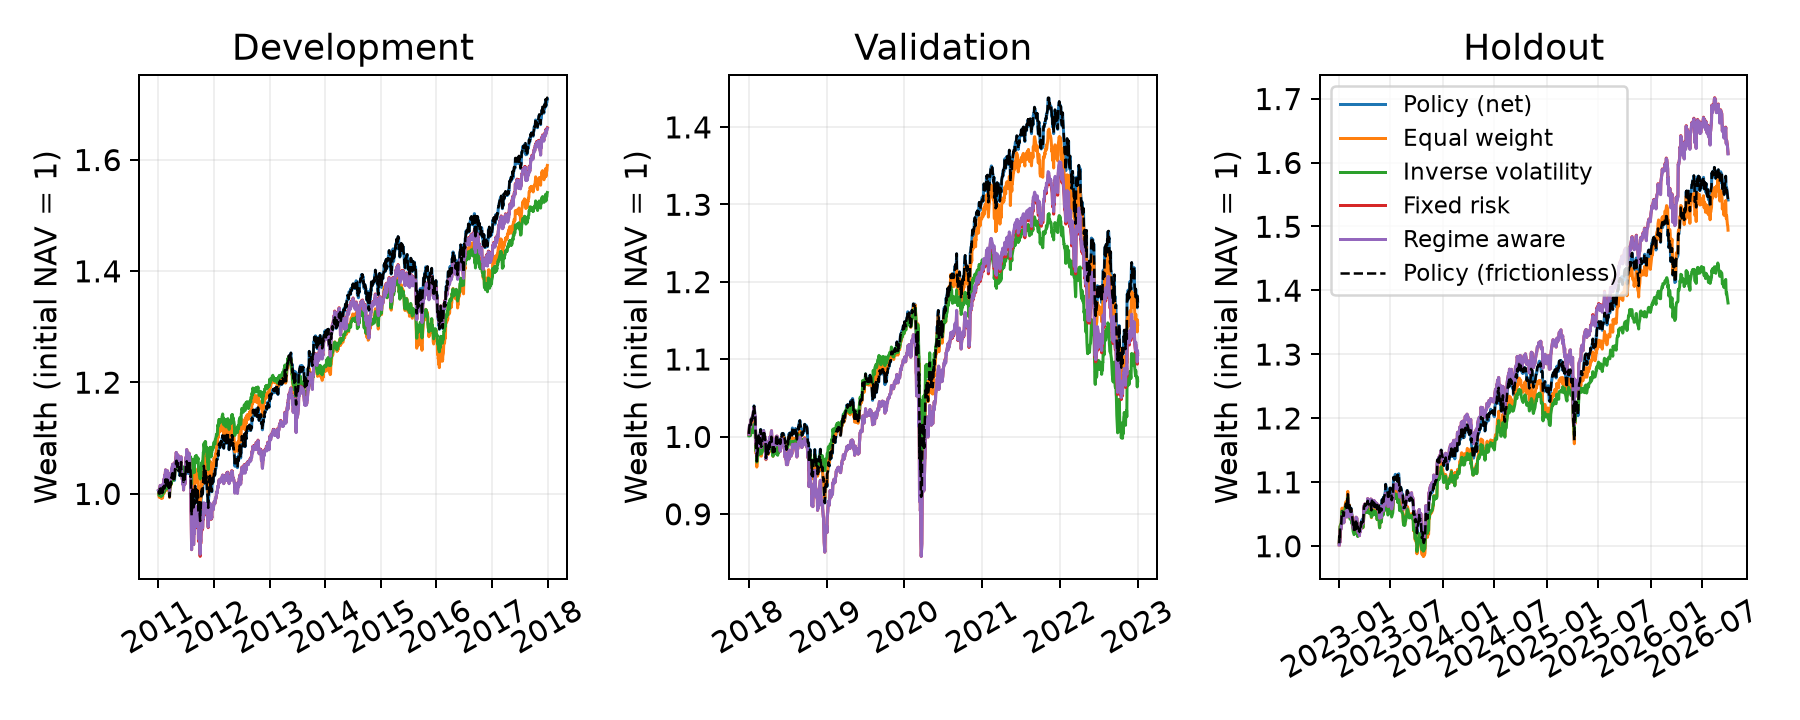
\includegraphics[width=\textwidth]{../results/empirical_phase2_reviewed/figures/wealth.png}
\caption{Executed cumulative net wealth with the frictionless policy shown separately. Each period is independently endowed at NAV 1.}
\end{figure}

\begin{figure}[htbp]\centering
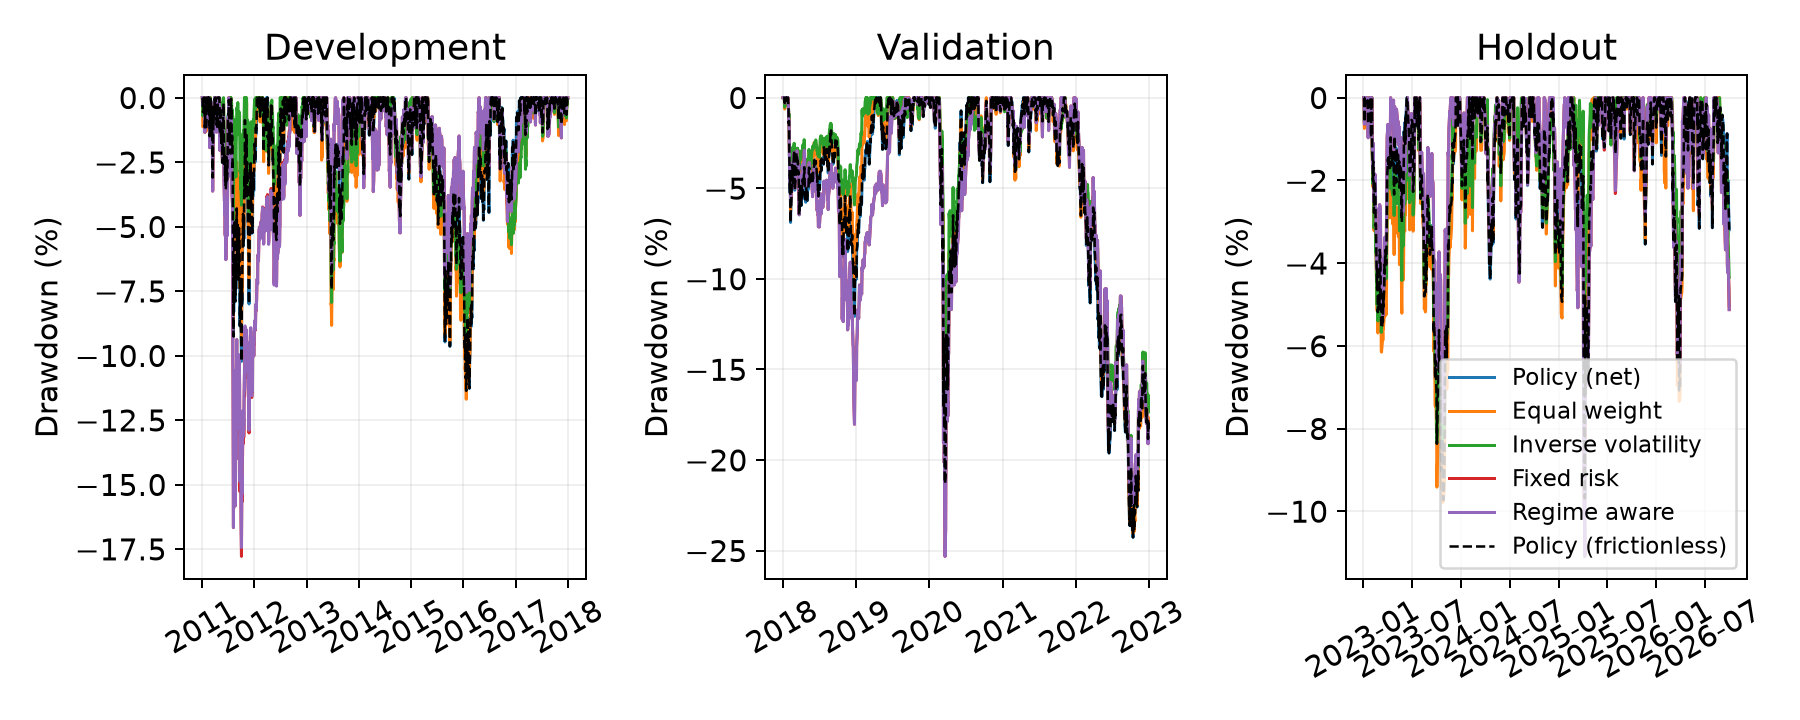
\includegraphics[width=\textwidth]{../results/empirical_phase2_reviewed/figures/drawdowns.png}
\caption{Executed net drawdowns, including initial NAV 1 in the running high-water mark.}
\end{figure}

\begin{figure}[htbp]\centering
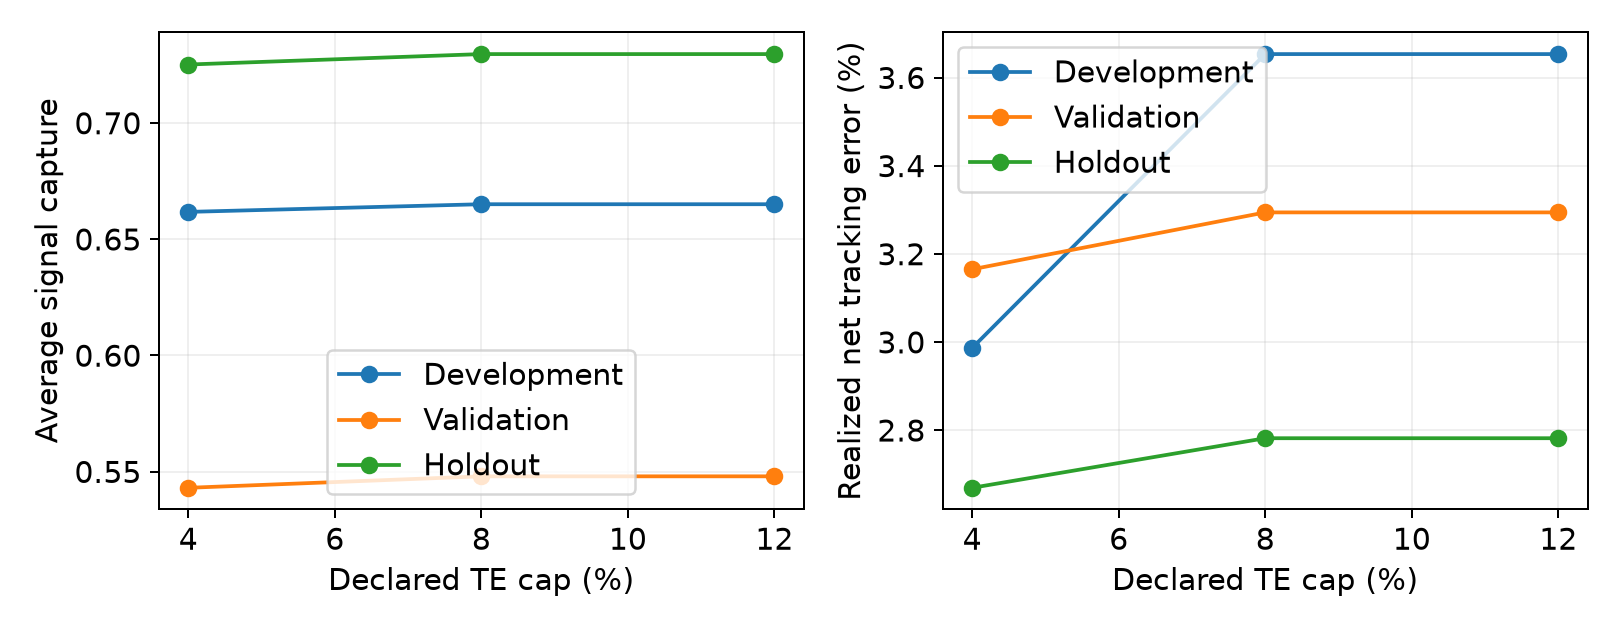
\includegraphics[width=\textwidth]{../results/empirical_phase2_reviewed/figures/te_frontier.png}
\caption{Declared TE mandates versus average signal capture and realized net TE; all other primary settings fixed.}
\end{figure}

\begin{figure}[htbp]\centering
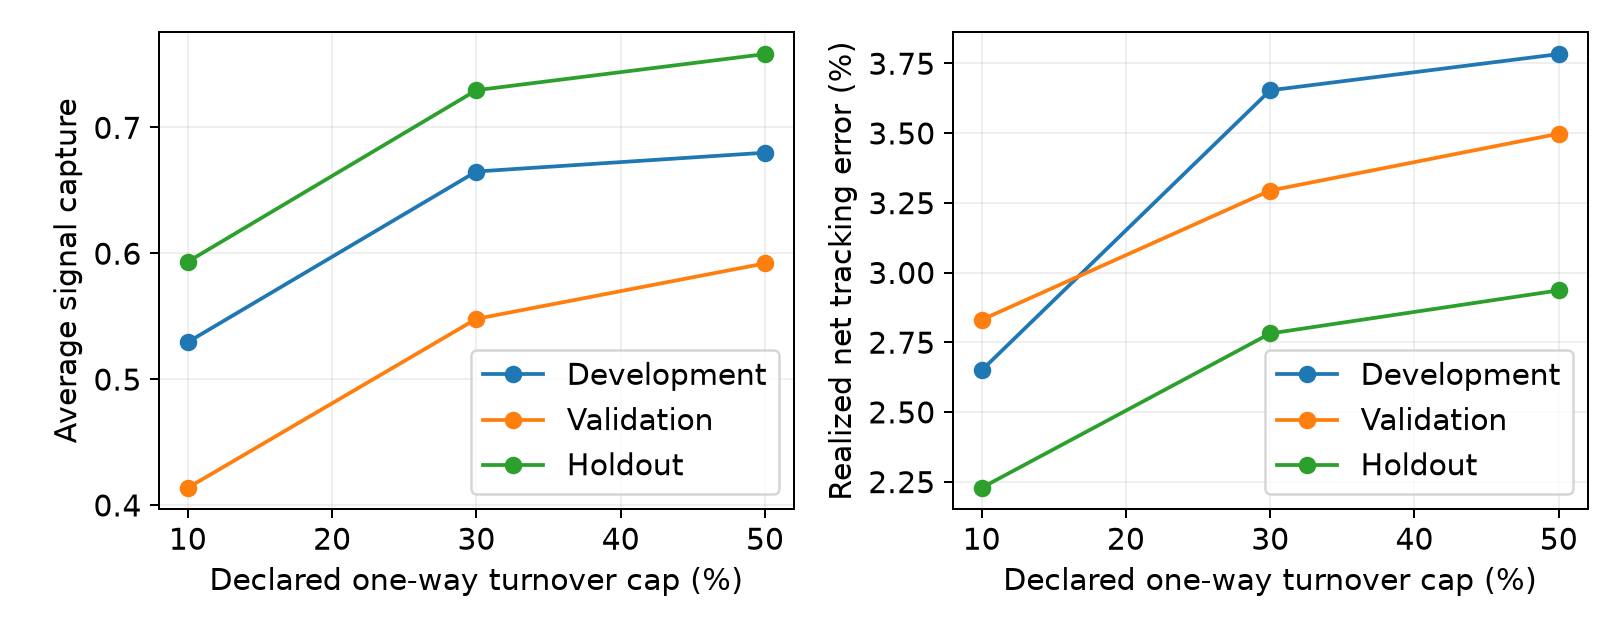
\includegraphics[width=\textwidth]{../results/empirical_phase2_reviewed/figures/turnover_frontier.png}
\caption{Declared turnover mandates versus capture and realized net TE; the identical two-percentage-point formation reserve applies throughout.}
\end{figure}

\begin{figure}[htbp]\centering
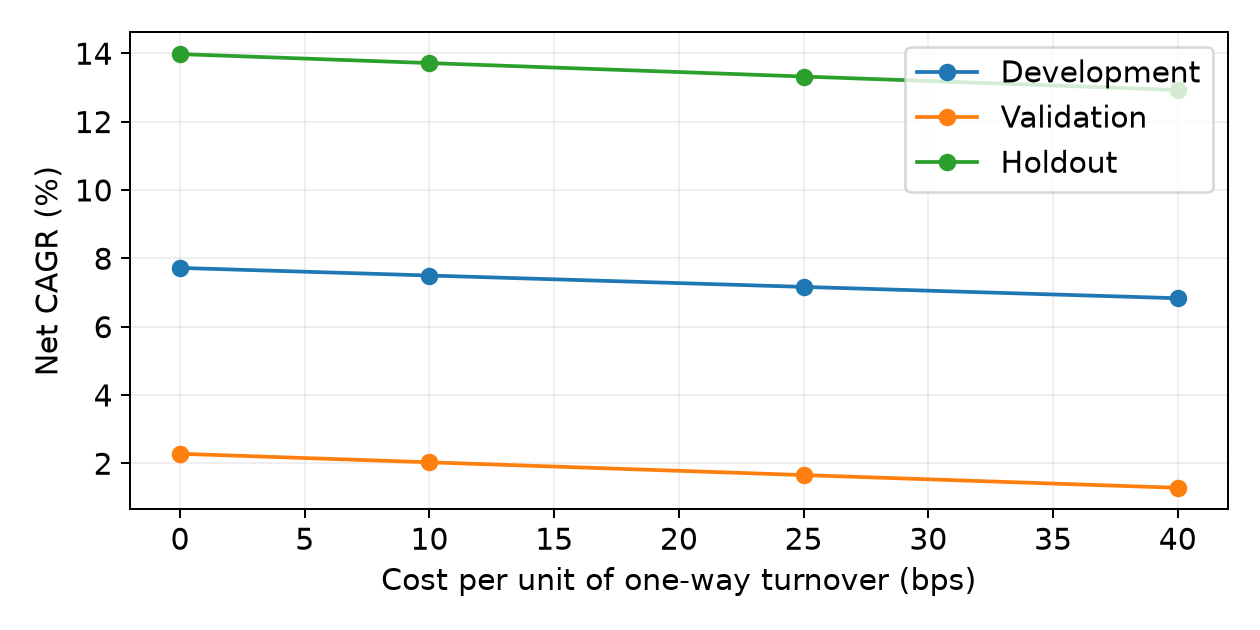
\includegraphics[width=\textwidth]{../results/empirical_phase2_reviewed/figures/cost_sensitivity.png}
\caption{Net CAGR under accounting-only cost changes with identical gross returns, holdings and trades.}
\end{figure}

\begin{figure}[htbp]\centering
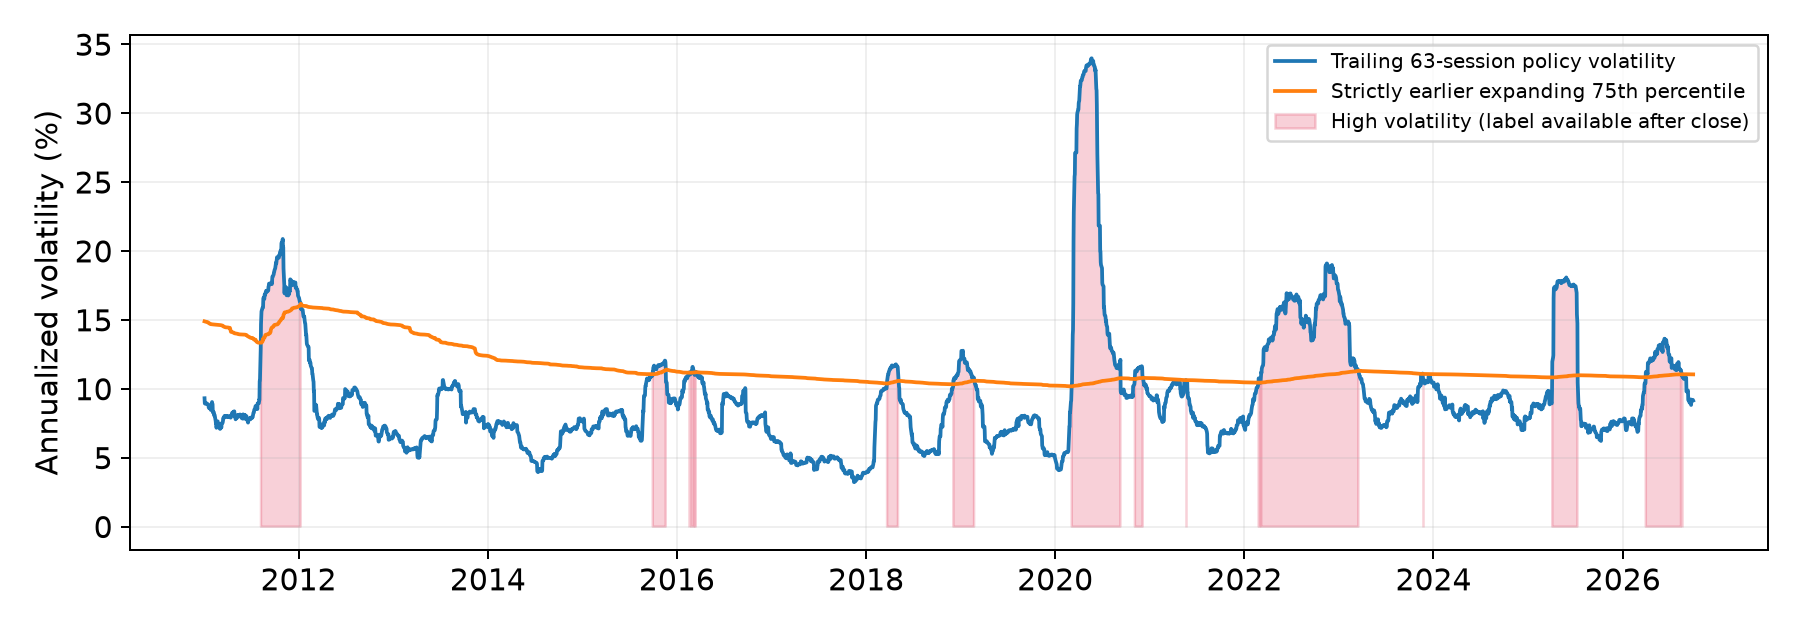
\includegraphics[width=\textwidth]{../results/empirical_phase2_reviewed/figures/regime_timeline.png}
\caption{Policy volatility and its strictly earlier expanding threshold. Red shading marks observation-date high-state labels, available only after that close.}
\end{figure}

\begin{figure}[htbp]\centering
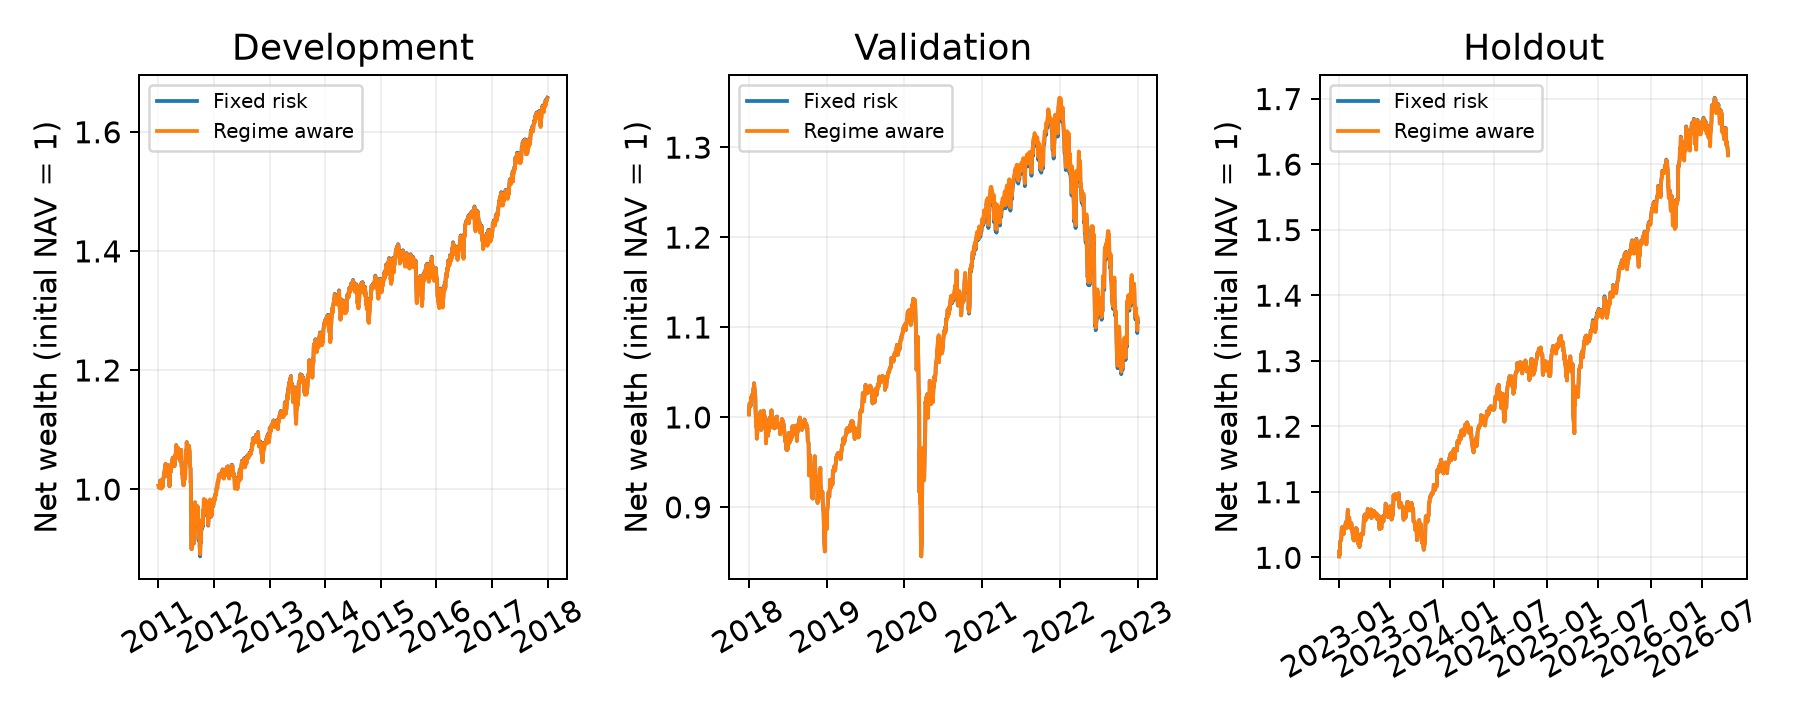
\includegraphics[width=\textwidth]{../results/empirical_phase2_reviewed/figures/fixed_vs_regime.png}
\caption{Executed fixed-risk and regime-aware net wealth; small visual differences need not indicate meaningful skill.}
\end{figure}

\begin{figure}[htbp]\centering
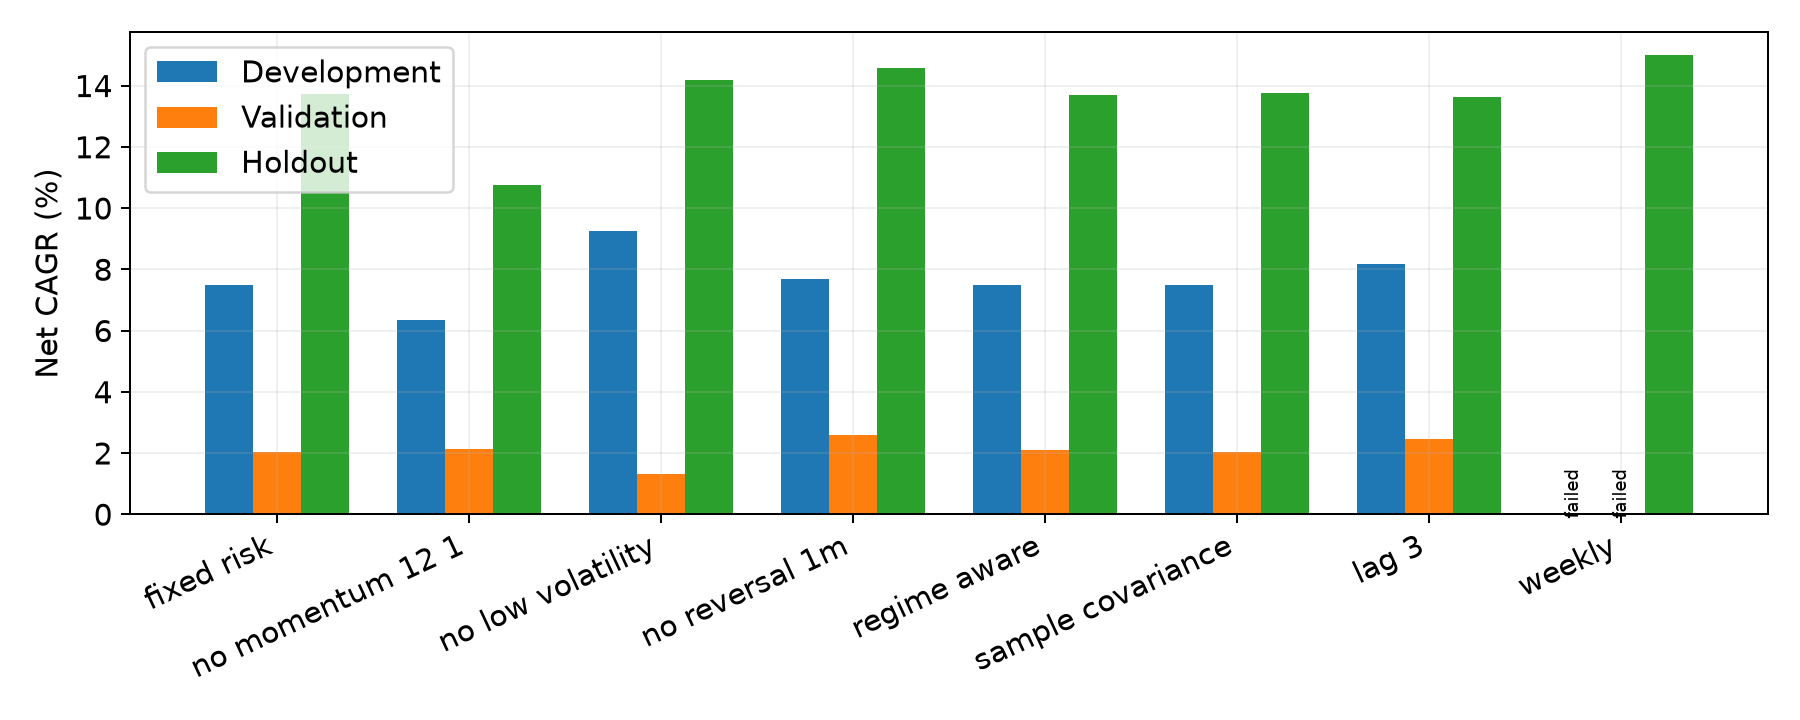
\includegraphics[width=\textwidth]{../results/empirical_phase2_reviewed/figures/ablation_robustness.png}
\caption{Executed ablations and robustness comparisons. Failed full-period paths have no return bar.}
\end{figure}


\clearpage
\begin{thebibliography}{9}
\raggedright
\bibitem{jt} Jegadeesh, N., and Titman, S. (1993). Returns to buying winners
and selling losers: Implications for stock market efficiency.
\emph{Journal of Finance} 48(1), 65--91.
\url{https://doi.org/10.1111/j.1540-6261.1993.tb04702.x}.
\bibitem{ang} Ang, A., Hodrick, R. J., Xing, Y., and Zhang, X. (2006).
The cross-section of volatility and expected returns.
\emph{Journal of Finance} 61(1), 259--299.
\url{https://doi.org/10.1111/j.1540-6261.2006.00836.x}.
\bibitem{lehmann} Lehmann, B. N. (1990). Fads, martingales, and market efficiency.
\emph{Quarterly Journal of Economics} 105(1), 1--28.
\url{https://doi.org/10.2307/2937816}.
\bibitem{lw} Ledoit, O., and Wolf, M. (2004). A well-conditioned estimator for
large-dimensional covariance matrices. \emph{Journal of Multivariate Analysis}
88(2), 365--411. \url{https://doi.org/10.1016/S0047-259X(03)00096-4}.
\bibitem{dgu} DeMiguel, V., Garlappi, L., and Uppal, R. (2009). Optimal versus
naive diversification: How inefficient is the 1/N portfolio strategy?
\emph{Review of Financial Studies} 22(5), 1915--1953.
\url{https://doi.org/10.1093/rfs/hhm075}.
\bibitem{kunsch} K\"unsch, H. R. (1989). The jackknife and the bootstrap for
general stationary observations. \emph{Annals of Statistics} 17(3), 1217--1241.
\url{https://doi.org/10.1214/aos/1176347265}.
\bibitem{tigzig} TigZig (2026). Yahoo Finance Data API documentation.
\url{https://www.tigzig.com/apis/yahoo-finance}. Accessed October 9, 2026.
\bibitem{terms} TigZig (2026). Terms of Use (August 2026 revision).
\url{https://www.tigzig.com/terms}. Accessed October 9, 2026.
\end{thebibliography}
\appendix
\section{All declared scenario results}
Table values are percentages for CAGR, active return, TE and turnover;
capture is unitless. A dash denotes an unavailable full-period metric.
Complete Sharpe, Sortino, volatility, drawdown, information ratio, wealth,
cost drag, active share, IC and constraint diagnostics are in
\texttt{all\_performance.csv} and the per-scenario ledgers.
\begin{center}\scriptsize
\begin{longtable}{llrrrrr}
\caption{All executed scenarios; failures are retained.}\label{allresults}\\
\toprule Period & Scenario & Net CAGR & Active & TE & Capture & Turnover\\\midrule\endfirsthead
\toprule Period & Scenario & Net CAGR & Active & TE & Capture & Turnover\\\midrule\endhead

development & fixed\_risk & 7.499 & -0.380 & 3.653 & 0.665 & 17.210\\

development & te\_4pct & 7.790 & -0.168 & 2.986 & 0.662 & 17.273\\

development & te\_8pct & 7.499 & -0.380 & 3.653 & 0.665 & 17.210\\

development & te\_12pct & 7.499 & -0.380 & 3.653 & 0.665 & 17.210\\

development & turnover\_10pct & 8.003 & 0.025 & 2.649 & 0.529 & 7.272\\

development & turnover\_30pct & 7.499 & -0.380 & 3.653 & 0.665 & 17.210\\

development & turnover\_50pct & 7.532 & -0.345 & 3.783 & 0.680 & 20.522\\

development & cost\_0bps & 7.722 & -0.173 & 3.651 & 0.665 & 17.210\\

development & cost\_10bps & 7.499 & -0.380 & 3.653 & 0.665 & 17.210\\

development & cost\_25bps & 7.166 & -0.690 & 3.658 & 0.665 & 17.210\\

development & cost\_40bps & 6.834 & -1.001 & 3.666 & 0.665 & 17.210\\

development & regime\_aware & 7.486 & -0.396 & 3.626 & 0.665 & 17.316\\

development & without\_momentum\_12\_1 & 6.351 & -1.581 & 2.386 & 0.419 & 17.198\\

development & without\_low\_volatility & 9.256 & 1.402 & 4.989 & 0.629 & 21.105\\

development & without\_reversal\_1m & 7.678 & -0.293 & 2.837 & 0.689 & 10.438\\

development & policy & 7.976 & -0.011 & 0.004 & -- & 0.885\\

development & equal\_weight & 6.859 & -1.082 & 2.462 & -- & 1.557\\

development & inverse\_volatility & 6.384 & -1.697 & 4.355 & -- & 4.241\\

development & sample\_covariance & 7.494 & -0.384 & 3.653 & 0.665 & 17.245\\

development & lag\_3 & 8.178 & 0.163 & 2.963 & 0.653 & 17.595\\

development & weekly & -- & -- & -- & -- & --\\

validation & fixed\_risk & 2.033 & -1.148 & 3.294 & 0.548 & 20.398\\

validation & te\_4pct & 2.203 & -0.979 & 3.165 & 0.543 & 19.746\\

validation & te\_8pct & 2.033 & -1.148 & 3.294 & 0.548 & 20.398\\

validation & te\_12pct & 2.033 & -1.148 & 3.294 & 0.548 & 20.398\\

validation & turnover\_10pct & 2.451 & -0.718 & 2.831 & 0.414 & 7.816\\

validation & turnover\_30pct & 2.033 & -1.148 & 3.294 & 0.548 & 20.398\\

validation & turnover\_50pct & 2.692 & -0.502 & 3.498 & 0.592 & 27.121\\

validation & cost\_0bps & 2.283 & -0.903 & 3.291 & 0.548 & 20.398\\

validation & cost\_10bps & 2.033 & -1.148 & 3.294 & 0.548 & 20.398\\

validation & cost\_25bps & 1.659 & -1.515 & 3.301 & 0.548 & 20.398\\

validation & cost\_40bps & 1.286 & -1.883 & 3.313 & 0.548 & 20.398\\

validation & regime\_aware & 2.086 & -1.093 & 3.250 & 0.546 & 19.938\\

validation & without\_momentum\_12\_1 & 2.143 & -1.108 & 3.547 & 0.385 & 19.809\\

validation & without\_low\_volatility & 1.312 & -1.765 & 4.989 & 0.576 & 20.635\\

validation & without\_reversal\_1m & 2.591 & -0.642 & 3.208 & 0.604 & 12.233\\

validation & policy & 3.271 & -0.013 & 0.004 & -- & 1.112\\

validation & equal\_weight & 2.743 & -0.618 & 2.752 & -- & 1.881\\

validation & inverse\_volatility & 1.400 & -2.228 & 5.436 & -- & 5.065\\

validation & sample\_covariance & 2.032 & -1.148 & 3.293 & 0.548 & 20.375\\

validation & lag\_3 & 2.463 & -0.745 & 3.276 & 0.534 & 21.237\\

validation & weekly & -- & -- & -- & -- & --\\

holdout & fixed\_risk & 13.717 & 1.233 & 2.782 & 0.730 & 19.135\\

holdout & te\_4pct & 13.231 & 0.786 & 2.669 & 0.725 & 18.822\\

holdout & te\_8pct & 13.717 & 1.233 & 2.782 & 0.730 & 19.135\\

holdout & te\_12pct & 13.717 & 1.233 & 2.782 & 0.730 & 19.135\\

holdout & turnover\_10pct & 14.216 & 1.639 & 2.228 & 0.593 & 7.338\\

holdout & turnover\_30pct & 13.717 & 1.233 & 2.782 & 0.730 & 19.135\\

holdout & turnover\_50pct & 13.508 & 1.040 & 2.936 & 0.758 & 22.762\\

holdout & cost\_0bps & 13.980 & 1.465 & 2.782 & 0.730 & 19.135\\

holdout & cost\_10bps & 13.717 & 1.233 & 2.782 & 0.730 & 19.135\\

holdout & cost\_25bps & 13.323 & 0.887 & 2.785 & 0.730 & 19.135\\

holdout & cost\_40bps & 12.931 & 0.540 & 2.792 & 0.730 & 19.135\\

holdout & regime\_aware & 13.700 & 1.218 & 2.773 & 0.729 & 19.198\\

holdout & without\_momentum\_12\_1 & 10.752 & -1.481 & 2.518 & 0.423 & 16.535\\

holdout & without\_low\_volatility & 14.202 & 1.891 & 4.250 & 0.594 & 20.959\\

holdout & without\_reversal\_1m & 14.577 & 2.005 & 2.951 & 0.807 & 10.956\\

holdout & policy & 12.315 & -0.009 & 0.003 & -- & 0.762\\

holdout & equal\_weight & 11.379 & -0.853 & 2.841 & -- & 1.886\\

holdout & inverse\_volatility & 9.034 & -3.160 & 3.746 & -- & 4.468\\

holdout & sample\_covariance & 13.762 & 1.273 & 2.785 & 0.730 & 19.142\\

holdout & lag\_3 & 13.640 & 1.140 & 2.777 & 0.738 & 19.189\\

holdout & weekly & 14.992 & 2.377 & 3.207 & 0.747 & 10.037\\

\bottomrule\end{longtable}\end{center}

Failure: development, weekly: Execution mandate failed on 2012-06-04: sector active weight, sector active weight.


Failure: validation, weekly: Execution mandate failed on 2020-03-16: sector active weight.


\section{Reproduction appendix}

Frozen code commit: \texttt{86a72b72584cf70e990525b62a7d4fab6e3649bd}.


Dataset SHA-256: \path{5af0b0c65a9b4f8be569090f974c0b5446839a0bac20c3485d2184109cf981ea}.



See \texttt{docs/empirical\_phase2.md} for the data-provider and issuer sources,
environment versions, original failures, exact commands and verification record.
\paragraph{Exact-input reproduction.}
The original bundle (original responses, prices, actions and manifest) is local
and not publicly distributed. Exact-input reproduction requires access to that
bundle, matching recorded fingerprints, the frozen model commit and protocol,
and compatible recorded dependencies. Numerical agreement is subject to solver
tolerances; byte-for-byte equality across environments is not promised.
The local validation reproduction and accounting audit used the original bundle;
they do not establish that an external reader can retrieve the same vintage.
Dataset hashes identify the inputs but cannot provide them.

\paragraph{Approximate replication with a new vintage.}
The acquisition commands retrieve fresh provider data, whose historical adjusted
prices or actions may have changed. This replicates the method, not necessarily
the published numerical results. Preserve a new manifest and fingerprints and
use a new explicitly labelled output directory. The original frozen holdout
output must not be overwritten or retuned. Public ledgers, tables and figures
support evidence inspection without supplying independent source-price reconstruction.
The reporting script reads executed
ledgers and never calls the optimizer. The manuscript compiles from the
repository root using the documented Tectonic command.
\end{document}
